
The LSST Camera was constructed at the SLAC National Accelerator Laboratory in California, US \citep{10.1117/12.3019302}.
The functionality and performance of the Camera had been studied in various integration phases from two rafts testing (Run 1; March 2019--April 2019 and Run 2; June 2019), nine rafts testing (Run 3; Oct 2019--Nov 2019), the full focal plane testing (Run4; Aug 2020--Nov 2020 and Jan 2020--Feb 2021), the full focal plane with the utility trunk (Run 5; Nov 2021--Jan 2022), and the full Camera testing (Run 6a; June 2023 and Run 6b; Oct 2023--Oct 2024). These testings verified the Camera functionality and led to discoveries of non-ideal features and means of mitigating many of them \citep{2024SPIE13096E..1SR}.

In May 2024,  the LSST Camera was loaded into a Boeing 747 airplane in San Francisco, CA, flown by air, and then transported by trucks from Santiago, Chile to the summit of Cerro Pachón at 2700\,m in the Andes mountain range in Chile, where the NFS-DOE Vera C. Rubin Observatory is being constructed. The LSST Camera was transferred from the truck to a support structure which was then rolled into the clean room, known as the White Room, on Level 3 of the Vera C. Rubin Observatory. After connecting lines for power and cooling and verifying the integrity of the vacuum, cool down began in late August. Following this, the seventh series of electro-optical (EO) testing, Run 7, prior to installation on the Telescope Mount Assembly (TMA), was conducted from the end of September 2024 to the beginning of December 2024 to reverify its performance and undertake further optimization. We collected 56,066 exposures during this testing campaign since the Camera became the full operational state (high voltages applied to CCDs) and the data were sent to the processing nodes at the SLAC Shared Scientific Data Facility (\textbf{S3DF}).

This document details initial interim testing results, with a focus on several points:
\begin{itemize}
    \item What is the difference of testing setup? (Section~\ref{sec:electro-optical-setup})
    \item Does the Camera after the transportation still perform as we checked out in California? (Section \ref{sec:reverification})
    \item Optimizations to the features that we found during previous EO testings such as persistence and bias instability. (Section \ref{sec:camera-optimization})
    \item How does the Camera perform after implementing those optimizations? (Section \ref{characterization-camera-stability})
    \item Investigating other features (Section \ref{sensor-features})
    \item Summarize the overall operations and issues during Run 7 (Section \ref{sec:issues})
\end{itemize}
All the results presented here are subject to future changes.

Figure \ref{fig:focal-plane-layout} shows the layout of the focal plane. The LSST focal plane consists of 21 Science Rafts and 4 Corner Rafts (cyan). Science Rafts have two varieties based on the vendor of the sensors used for the Raft: ITL (green) or e2v (yellow). Each sensor has 4k$\times$4k pixels, segmented by 16 channels to make the fastest readout being 2 seconds. Corner Rafts have two different kinds of sensors: guider sensors and a wavefront sensor. Guider sensors are ITL sensors as are some of the other science sensors, while the wavefront sensor is an ITL sensor split in the middle and packaged into one sensor with an offset by $\pm2$mm with respect to the other science sensors to provide off-focus point source images to measure ``donuts" -- an image of the pupil used to regulate the focus of the telescope.
\begin{figure}
    \centering
    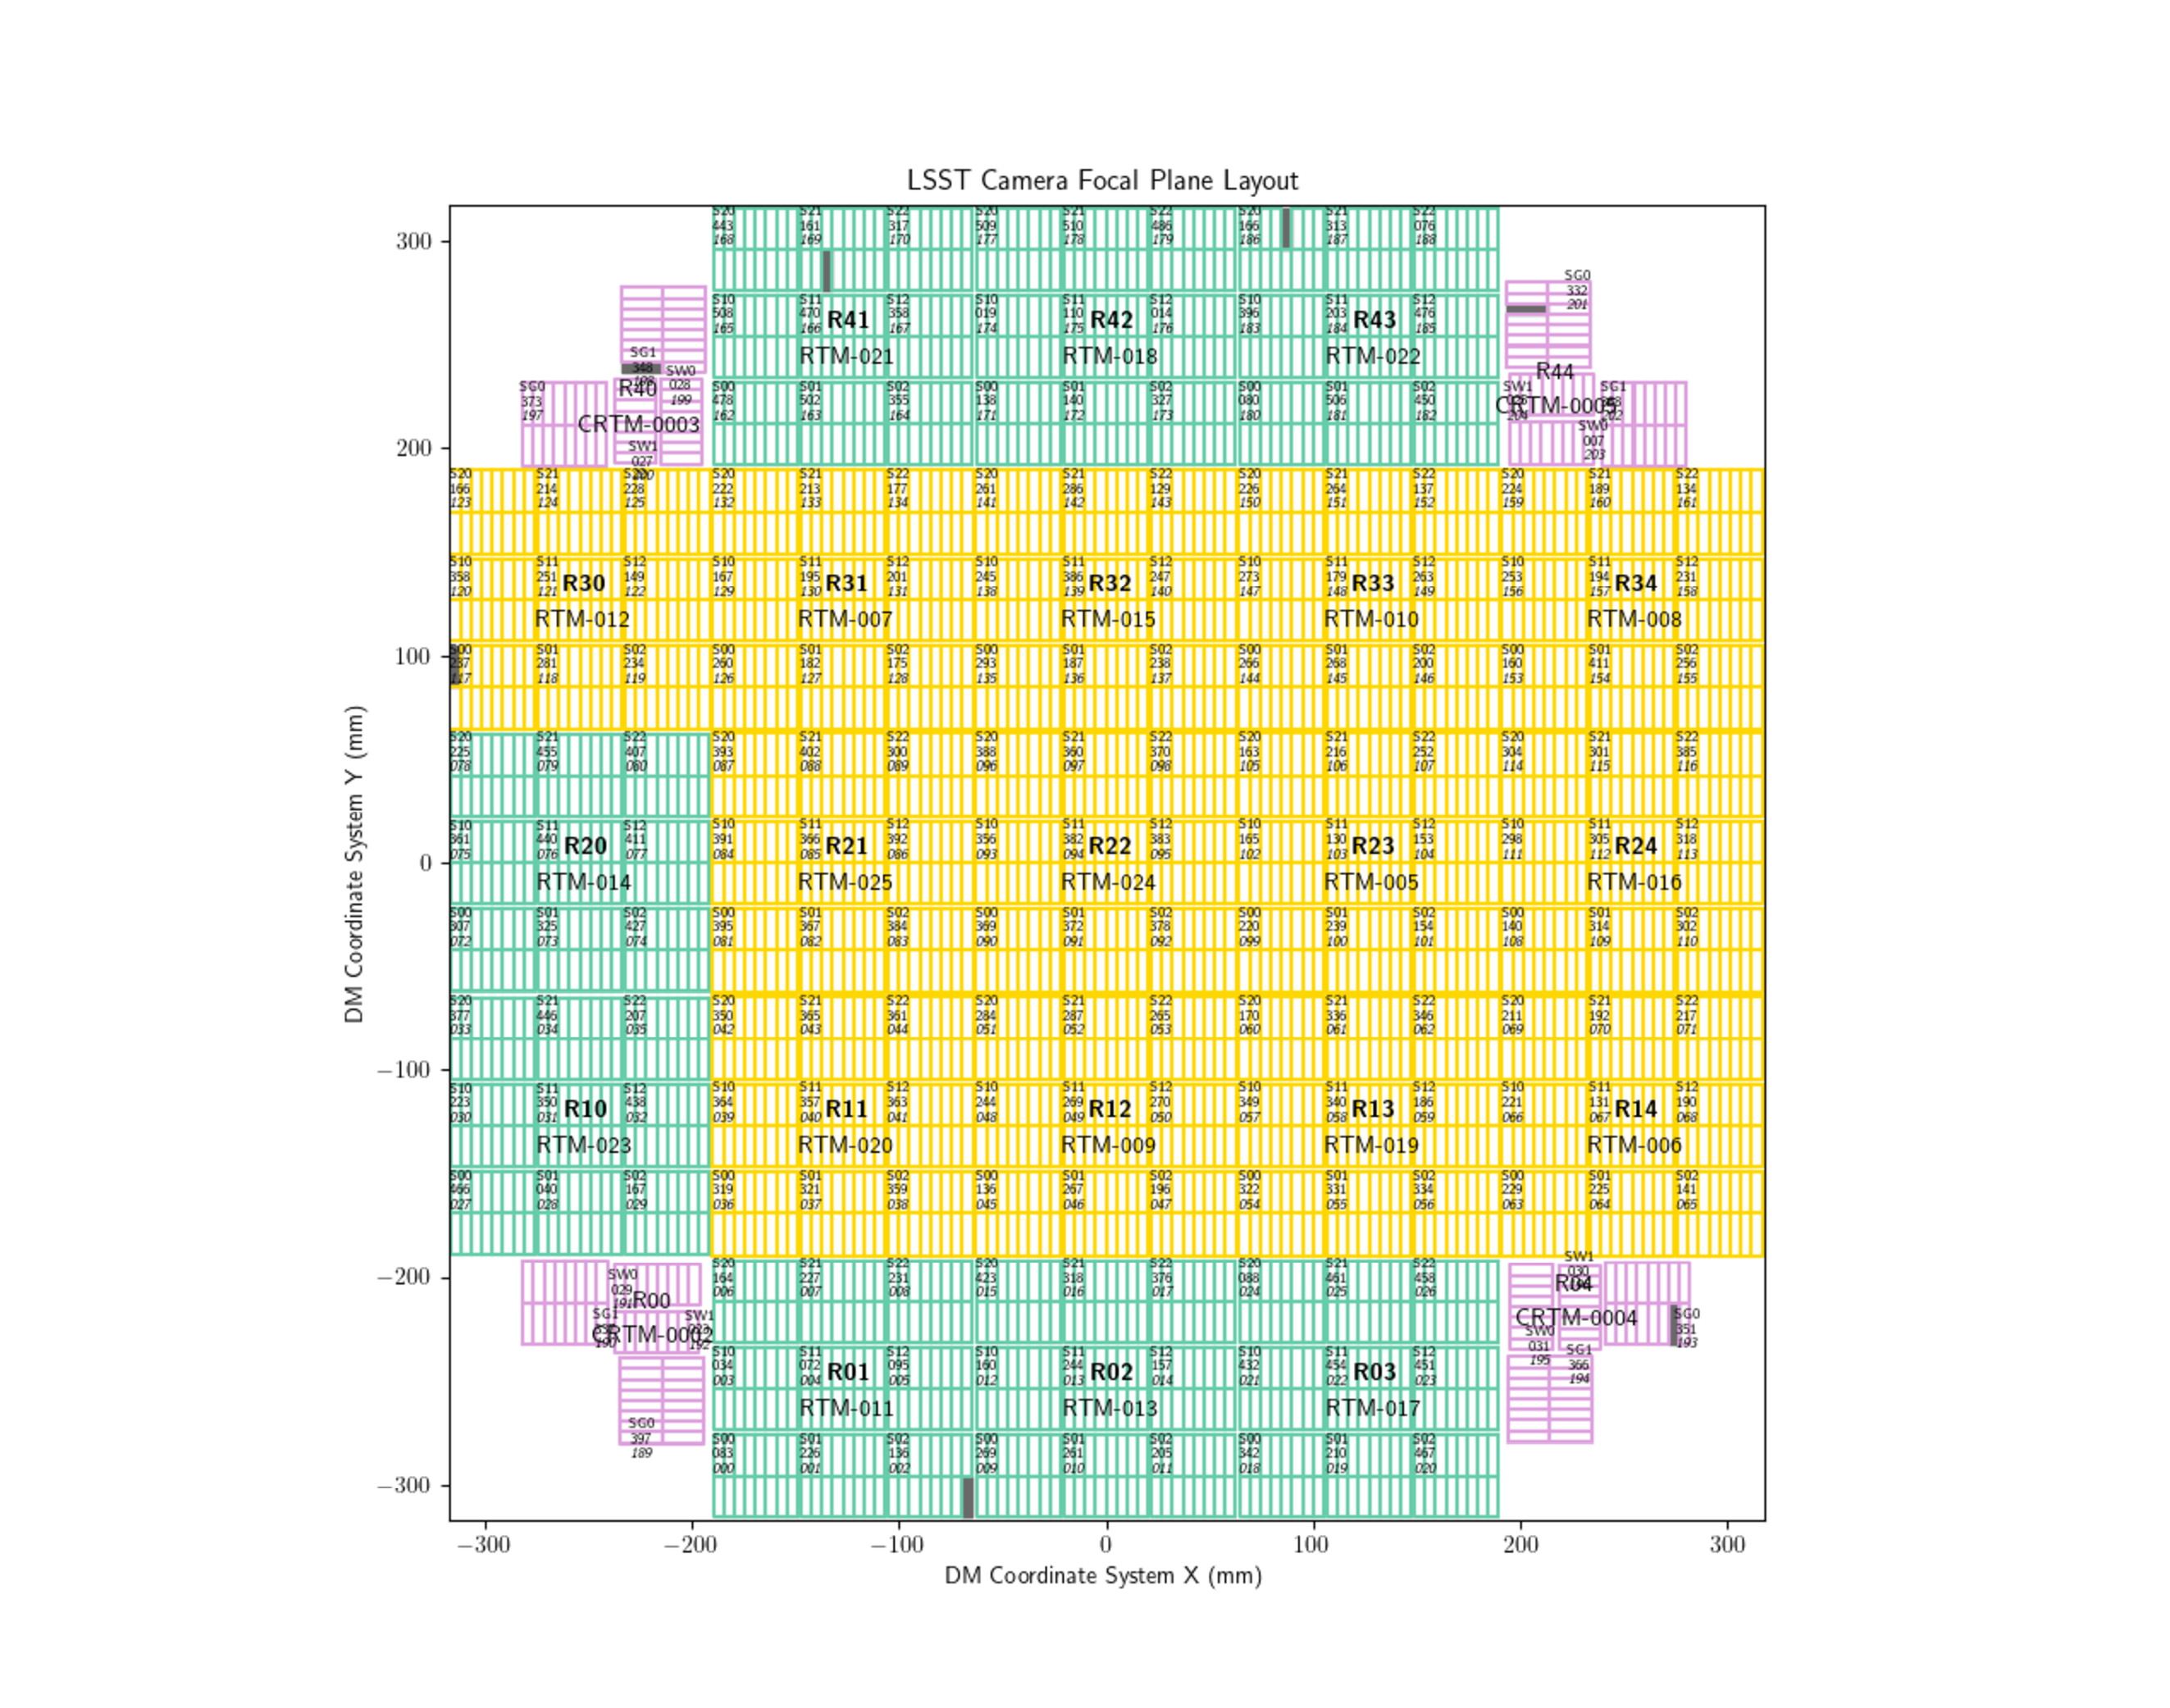
\includegraphics[width=1.0\linewidth]{figures/introduction/LSSTCam_fp_layout_Oct2024.pdf}
    \caption{The focal plane layout}
    \label{fig:focal-plane-layout}
\end{figure}

\clearpage